%%%%%%%%%%%%%%%%%%%%%%%%%%%%%%%%%%%%%%%%%%%%%%%%%%%%%%%%%%%%%%%%%
% MUW Presentation
% LaTeX Template
% Version 1.0 (27/12/2016)
%
% License:
% CC BY-NC-SA 4.0 (http://creativecommons.org/licenses/by-nc-sa/3.0/)
%
% Created by:
% Nicolas Ballarini, CeMSIIS, Medical University of Vienna
% nicoballarini@gmail.com
% http://statistics.msi.meduniwien.ac.at/
%%%%%%%%%%%%%%%%%%%%%%%%%%%%%%%%%%%%%%%%%%%%%%%%%%%%%%%%%%%%%%%%%
\documentclass[8pt,pdf,hyperref={unicode}, xcolor=dvipsnames, fleqn]{beamer}
\usepackage{array} % Для титульника
\usepackage{ucs}
\usepackage[utf8x]{inputenc} % Включаем поддержку UTF8

%%%%XeLaTex part%%%
\usepackage{polyglossia}   %% загружает пакет многоязыковой вёрстки
\setdefaultlanguage{russian}  %% устанавливает главный язык документа
\setotherlanguage{english} %% объявляет второй язык документа
\defaultfontfeatures{Ligatures={TeX}}  %% свойства шрифтов по умолчанию
\setmainfont[Ligatures={TeX,Historic}]{Times New Roman} %% задаёт основной шрифт документа
\setsansfont{Arial}                    %% задаёт шрифт без засечек
\setmonofont{Courier New}               %% задаёт моноширинный шрифт
\newfontfamily{\cyrillicfonttt}{Courier New} % моноширинный шрифт, на который не ругается компилятор

\usetheme{MUW}
\usecolortheme{MUW}
\setbeamertemplate{navigation symbols}{} 
\setbeamertemplate{caption}[numbered]

%%%%%%%%%%%%%%%%%%%Button settings%%%%%%%%%%%%%%%%
%\definecolor{light-gray}{gray}{0.95}
%\setbeamercolor{button}{bg=white,fg=black}

%%%%%%%%%%%%%%%Список литературы
\usepackage[square, numbers, sort&compress]{natbib}
\newcommand{\empline}{\mbox{}\newline}
\renewcommand{\bibnumfmt}[1]{#1.\hfill}
%\renewcommand{\bibsection}{\chapter{ {\LARGE Список литературы}}}

\setlength{\bibsep}{0pt}
%%%%%%%%%%%%%%%Список литературы


%%%%%%%%%%%%%%%%%%%%%%%%%%%%%%%%%%%%%%%%%%%%%%%%%%%%%%%%%%%%%%%%%
%% Presentation Info
\title[Введение в Numpy и Jupyter notebook]{\textit{Занятие 2}: ~\\ Введение в Numpy и Jupyter notebook}
\author{ФКН}
\institute{Воронежский государственный университет}
\date{

	


			
}
%%%%%%%%%%%%%%%%%%%%%%%%%%%%%%%%%%%%%%%%%%%%%%%%%%%%%%%%%%%%%%%%%


%%%%%%%%%%%%%%%%%%%%%%%%%%%%%%%%%%%%%%%%%%%%%%%%%%%%%%%%%%%%%%%%%
%% FOOTLINE
%% Comment/Uncomment the following blocks to modify the footline
%% content in the body slides. 


%% Option A: Title and institute
%\footlineA
%% Option B: Author and institute
%\footlineB
%% Option C: Title, Author and institute
\footlineC
%%%%%%%%%%%%%%%%%%%%%%%%%%%%%%%%%%%%%%%%%%%%%%%%%%%%%%%%%%%%%%%%%

\begin{document}

%%%%%%%%%%%%%%%%%%%%%%%%%%%%%%%%%%%%%%%%%%%%%%%%%%%%%%%%%%%%%%%%%
% Use this block for a blue title slide with modified footline
{\titlepageBlue
\begin{frame}
  \titlepage
\end{frame}
}


%%%%%%%%%%%%%%%%%%%%%%%%%%%%%%%%%%%%%%%%%%%%%%%%%%%%%%%%%%%%%%%%%
% Comment/Uncomment these lines for an automatically generated outline.
%\begin{frame}{Outline}
%  \tableofcontents
%\end{frame}



%%%%%%%%%%%%%%%%%%%%%%%%%%%%%%%%%%%%%%%%%%%%%%%%%%%%%%%%%%%%%%%%%
\section{Введение}
\begin{frame}{Jupyter notebook}

Ранее рассматривался пакет Anaconda. Напомним, что он включает в себя сотни популярных библиотек для языка Python и работает на Windows, Linux и MacOS. Conda позволяет быстро и легко запускать и модернизировать проекты, использующие scikit-learn, TensorFlow, SciPy и многое другое. Помимо того, в её состав входит Jupyter Notebook, который в дальнейшем будет использоваться для работы. Рассмотрим его интерфейс более подробно:

\begin{figure}
	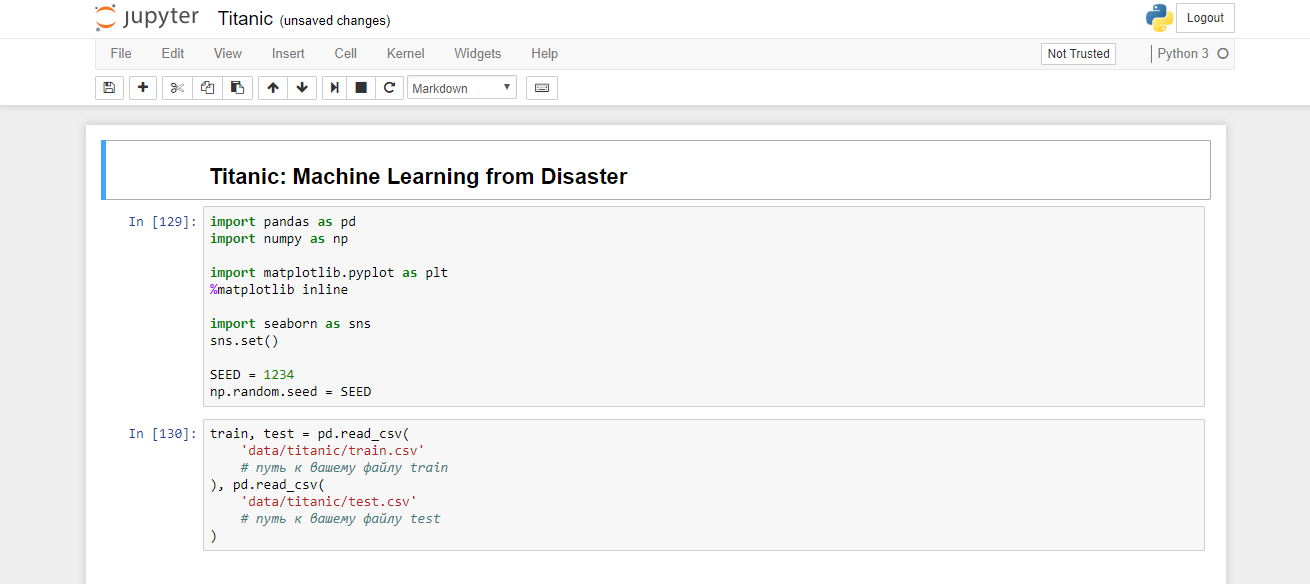
\includegraphics[width=1.0\textwidth]{Images/jupyter.png}
	%\caption{Пример типового листинга на языке Python в Visual Studio Code}
\end{figure}


\end{frame}
%%%%%%%%%%%%%%%%%%%%%%%%%%%%%%%%%%%%%%%%%%%%%%%%%%%%%%%%%%%%%%%%%
%%%%%%%%%%%%%%%%%%%%%%%%%%%%%%%%%%%%%%%%%%%%%%%%%%%%%%%%%%%%%%%%%
%%%%%%%%%%%%%%%%%%%%%%%%%%%%%%%%%%%%%%%%%%%%%%%%%%%%%%%%%%%%%%%%%
\begin{frame}{Основные особенности использования}

\begin{itemize}
	\item Jupyter представляет информацию в браузере, а выполняет вычисления средствами компьютера (эти действия можно наблюдать в терминале).
	\item Структура файла \textit{.ipynb} состоит из отдельных блоков нескольких видов. Нас будут интересовать: текст, он же Markdown (включая MD разметку, html и Latex вставки) и Code (блок, в котором можно писать код).
	\item Ctrl + Enter — выполнить строчку. Shift + Enter — выполнить строчку и перейти на следующую.
	\item Можно с помощью кнопок сверху создавать новые блоки (insert cell below), перемещать стрелками и удалять (удаление традиционно осуществляется через cut selected cells). Также существуют клавиатурные комбинации.
	\item Знак звёздочки (*) слева от блока означает, что он выполняется и, соответственно, цифра означает порядок, которым он был выполнен ранее.
	\item Установив курсор на импортированную функцию, можно нажать Shift+Tab и получить краткую справку по ней. Нажав еще раз, можно получить более полную справку.
	\item По умолчанию корневая директория сохранения файлов \textit{.ipynb} это $ C:\backslash Users\backslash \%username\% $.
	\item Дважды кликнув по ячейке, её можно отредактировать.
\end{itemize}


\end{frame}
%%%%%%%%%%%%%%%%%%%%%%%%%%%%%%%%%%%%%%%%%%%%%%%%%%%%%%%%%%%%%%%%%
%%%%%%%%%%%%%%%%%%%%%%%%%%%%%%%%%%%%%%%%%%%%%%%%%%%%%%%%%%%%%%%%%
\begin{frame}{Установка дополнительных библиотек}

Конечно же, может возникнуть ситуация, когда при решении той или иной задачи на компьютере будет отсутствовать какая-либо необходимая библиотека. Решить данную проблему можно, как правило, одним из двух способов. Для примера, установить через терминал \textit{numpy, scipy, pandas и sklearn} можно следующими вариантами:

\begin{itemize}
	\item python -m pip install numpy scipy pandas sklearn
	\item conda install numpy scipy pandas sklearn
\end{itemize}
Причём возможно установка удастся одним образом и не удастся вторым. Также могут возникнуть какие-либо иные ошибки при установке, специфичные для конкретной библиотеки. Их решение можно найти в документации к библиотеке или на StackOverflow.

\end{frame}
%%%%%%%%%%%%%%%%%%%%%%%%%%%%%%%%%%%%%%%%%%%%%%%%%%%%%%%%%%%%%%%%%
%%%%%%%%%%%%%%%%%%%%%%%%%%%%%%%%%%%%%%%%%%%%%%%%%%%%%%%%%%%%%%%%%
\begin{frame}{Использование NumPy}

\textbf{Numpy} позволяет быстро обрабатывать массивы и матрицы. Рассмотрим простейшие примеры использования

\begin{figure}
	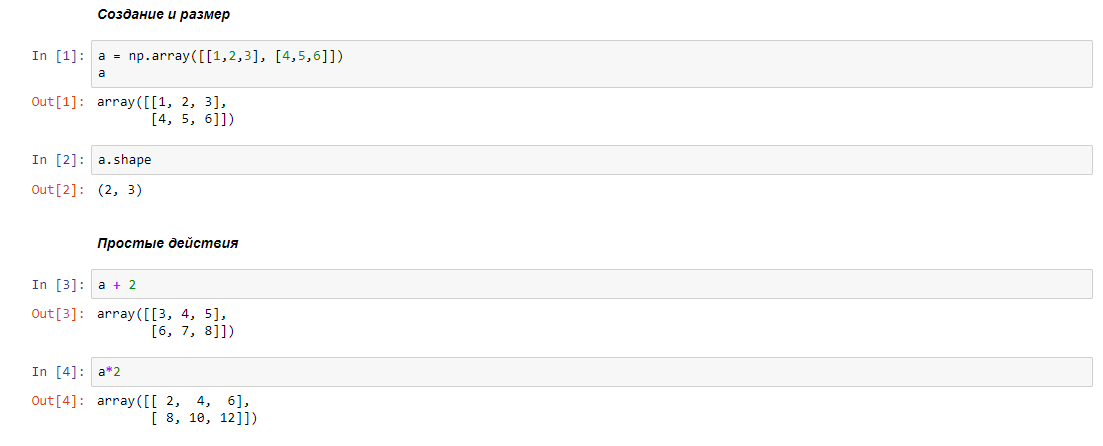
\includegraphics[width=1.0\textwidth]{Images/main1.png}
	%\caption{Пример типового листинга на языке Python в Visual Studio Code}
\end{figure}

\end{frame}
%%%%%%%%%%%%%%%%%%%%%%%%%%%%%%%%%%%%%%%%%%%%%%%%%%%%%%%%%%%%%%%%%
%%%%%%%%%%%%%%%%%%%%%%%%%%%%%%%%%%%%%%%%%%%%%%%%%%%%%%%%%%%%%%%%%
\begin{frame}{}


\begin{figure}
	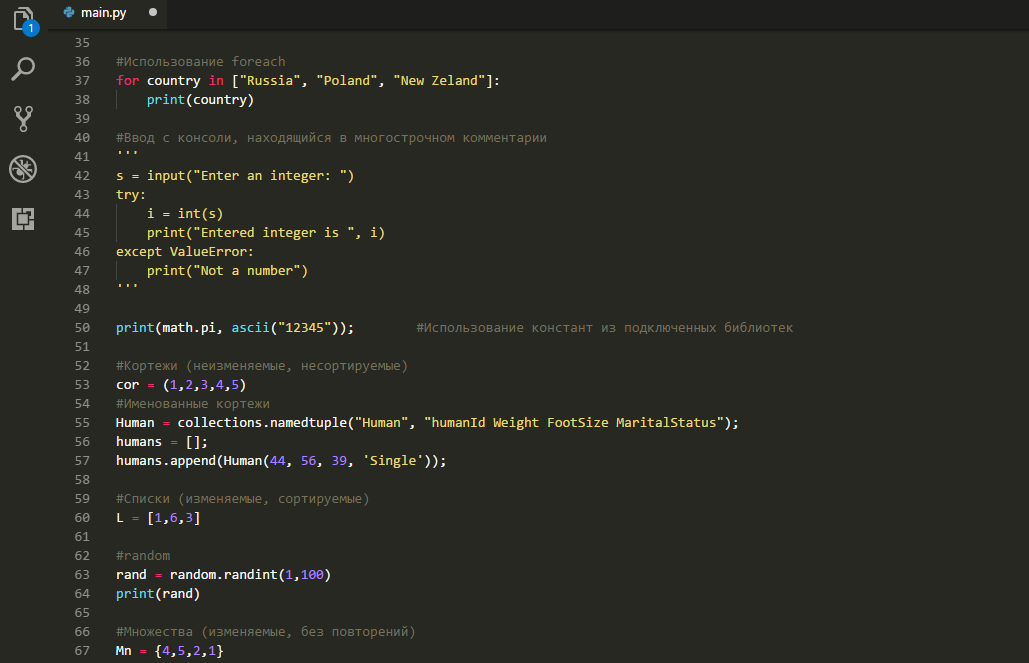
\includegraphics[width=1.0\textwidth]{Images/main2.png}
	%\caption{Пример типового листинга на языке Python в Visual Studio Code}
\end{figure}

\end{frame}
%%%%%%%%%%%%%%%%%%%%%%%%%%%%%%%%%%%%%%%%%%%%%%%%%%%%%%%%%%%%%%%%%
%%%%%%%%%%%%%%%%%%%%%%%%%%%%%%%%%%%%%%%%%%%%%%%%%%%%%%%%%%%%%%%%%
\begin{frame}{}


\begin{figure}
	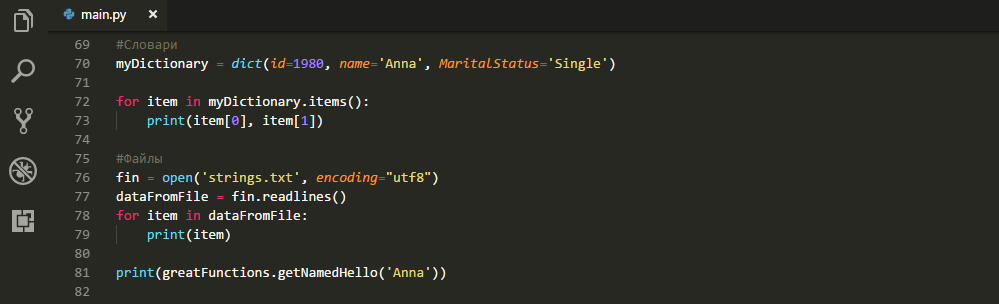
\includegraphics[width=1.0\textwidth]{Images/main3.png}
	%\caption{Пример типового листинга на языке Python в Visual Studio Code}
\end{figure}

\end{frame}
%%%%%%%%%%%%%%%%%%%%%%%%%%%%%%%%%%%%%%%%%%%%%%%%%%%%%%%%%%%%%%%%%
%%%%%%%%%%%%%%%%%%%%%%%%%%%%%%%%%%%%%%%%%%%%%%%%%%%%%%%%%%%%%%%%%
\begin{frame}{}
\begin{figure}
	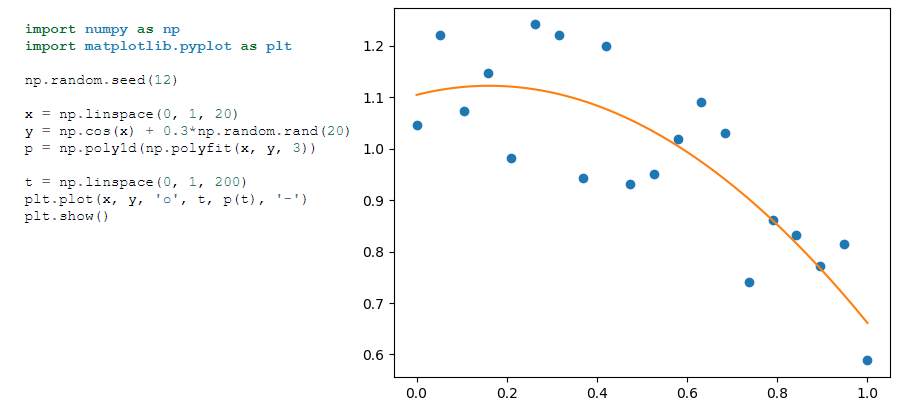
\includegraphics[width=1.0\textwidth]{Images/main4.png}
	%\caption{Пример типового листинга на языке Python в Visual Studio Code}
\end{figure}

\end{frame}
%%%%%%%%%%%%%%%%%%%%%%%%%%%%%%%%%%%%%%%%%%%%%%%%%%%%%%%%%%%%%%%%%
%%%%%%%%%%%%%%%%%%%%%%%%%%%%%%%%%%%%%%%%%%%%%%%%%%%%%%%%%%%%%%%%%
\begin{frame}{Библиотека SciPy}
\textbf{SciPy} - библиотека для языка программирования Python с открытым исходным кодом, предназначенная для выполнения научных и инженерных расчётов. Она может использоваться для поиска минимумов и максимумов функций, вычисления интегралов функций, обработки сигналов, обработки изображений, решения обыкновенных дифференциальных уравнений и т.д. Работает он на базе NumPy.

\begin{figure}
	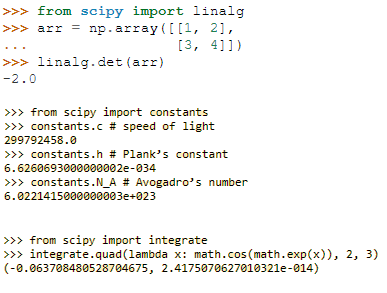
\includegraphics[width=0.7\textwidth]{Images/scipy.png}
	%\caption{Пример типового листинга на языке Python в Visual Studio Code}
\end{figure}

\end{frame}
%%%%%%%%%%%%%%%%%%%%%%%%%%%%%%%%%%%%%%%%%%%%%%%%%%%%%%%%%%%%%%%%%
%%%%%%%%%%%%%%%%%%%%%%%%%%%%%%%%%%%%%%%%%%%%%%%%%%%%%%%%%%%%%%%%%
\begin{frame}{Практические задания}


\begin{figure}
	
\includegraphics[width=1.0\textwidth]{Images/codingtime.jpg}
	%\caption{Пример типового листинга на языке Python в Visual Studio Code}
\end{figure}

\begin{enumerate}
	\item Запустить задание с прошлого занятия в Jupyter notebook
	\item Реализовать в Jupyter notebook алгоритм сортировки пузырьком и протестировать для ряда чисел: $ 92,11,45,2234,0,7,65 $
\end{enumerate}

\end{frame}
%%%%%%%%%%%%%%%%%%%%%%%%%%%%%%%%%%%%%%%%%%%%%%%%%%%%%%%%%%%%%%%%%
%%%%%%%%%%%%%%%%%%%%%%%%%%%%%%%%%%%%%%%%%%%%%%%%%%%%%%%%%%%%%%%%%
\begin{frame}{Ответы на задания}


\begin{figure}
	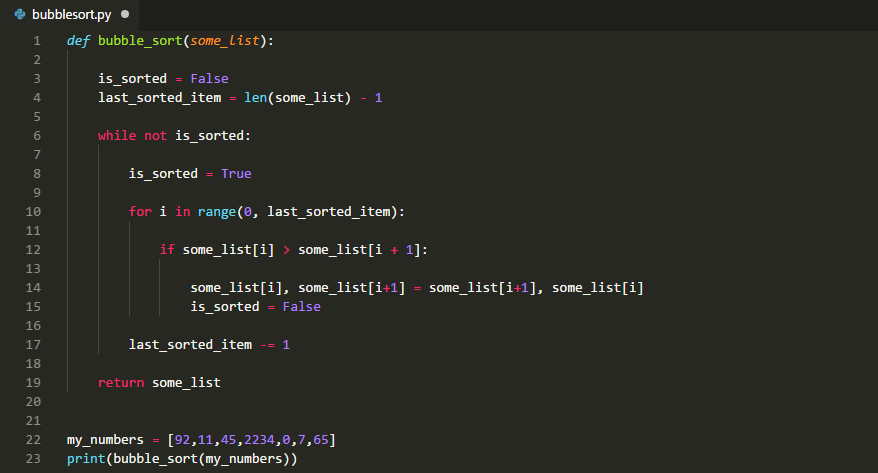
\includegraphics[width=1.0\textwidth]{Images/res.PNG}
	%\caption{Пример типового листинга на языке Python в Visual Studio Code}
\end{figure}


\end{frame}
%%%%%%%%%%%%%%%%%%%%%%%%%%%%%%%%%%%%%%%%%%%%%%%%%%%%%%%%%%%%%%%%%









\end{document}